\chapter{\MakeUppercase{Working Principle}}
\setcounter{equation}{0}

\section{{Motivation and Objectives}}

The main motivation for the selected research arises from the observation that stroke patients respond differently to Brain--Computer Interface (BCI) rehabilitation. Although BCI-based rehabilitation can support lower-limb motor recovery, some patients experience greater improvement than others. Therefore, predicting treatment response before rehabilitation can help clinicians understand individual recovery potential and plan appropriate treatment strategies.

To address this problem, the authors developed a prediction framework using multimodal behavioral data collected from 42 subacute stroke patients. The data included demographic, clinical, and biomechanical characteristics measured before rehabilitation. Machine learning and statistical models were used to investigate the relationship between these initial characteristics and the patient's motor function after two weeks of BCI treatment.

The main objectives are to predict post-treatment lower-limb motor function, classify patients as responders or non-responders, compare the performance of different prediction models, and identify the factors that contribute most to the predictions. Explainable Artificial Intelligence (XAI) techniques are used to make the model outputs more understandable and potentially useful for clinical decision-making \cite{bib1}.

\section{{Collection and Preparation of Patient Data}}

The proposed framework begins with the collection of patient information before BCI rehabilitation. The study used records from a larger assessor-blinded randomized controlled trial involving 167 participants. After selecting patients who received BCI therapy and excluding records with incomplete information for the required clinical assessments, 42 patients were included in the analysis \cite{bib1}.

\subsection{{Demographic Data}}

Demographic information describes the basic characteristics of each patient. The study considered four demographic features:

\begin{itemize}
    \item Age
    \item Sex
    \item Stroke type
    \item Time since stroke onset
\end{itemize}

These features help investigate whether differences in patient characteristics are associated with lower-limb motor recovery following BCI treatment.

\subsection{{Clinical Assessment Data}}

Clinical measurements provide information about the patient's initial motor function, muscle spasticity, balance, walking ability, and independence in daily activities. The study included eight clinical features:

\begin{itemize}
    \item Fugl-Meyer Assessment of the Lower Extremity (FMA-LE)
    \item Modified Ashworth Scale (MAS)
    \item Berg Balance Scale (BBS)
    \item Postural Assessment Scale for Stroke Patients (PASS)
    \item Bobath Level 3 Balance Rating (BBR)
    \item Six-Minute Walking Test (6MWT)
    \item Modified Barthel Index (MBI)
    \item Functional Ambulation Category (FAC)
\end{itemize}

These measurements help describe the patient's functional condition before treatment and provide potential predictors of the outcome after rehabilitation.

\subsection{{Biomechanical Data}}

Biomechanical measurements provide information about ankle movement and muscle strength. The study included six biomechanical features:

\begin{itemize}
    \item Dorsiflexion active range of motion (AROM)
    \item Dorsiflexion passive range of motion (PROM)
    \item Plantarflexion AROM
    \item Plantarflexion PROM
    \item Dorsiflexor muscle strength
    \item Plantarflexor muscle strength
\end{itemize}

These measurements help examine whether joint mobility and muscle strength contribute additional information when predicting treatment outcomes.

In total, the study used 18 baseline features from demographic, clinical, and biomechanical categories. These measurements were collected before the two-week BCI rehabilitation programme and used as inputs to the prediction models \cite{bib1}.

\section{{BCI Rehabilitation System}}

The patients underwent lower-limb Brain--Computer Interface rehabilitation (BCI-LE) for two weeks. The system combined an electroencephalography (EEG) acquisition device, signal-processing software, and an ankle-stretching rehabilitation robot.

\subsection{{EEG Signal Acquisition}}

A 64-channel wireless EEG system was used to record the patient's brain activity. During the calibration session, patients performed motor-imagery tasks in which they attempted to imagine dorsiflexing their ankle. The EEG signals were recorded during task and resting conditions.

\subsection{{Signal Processing and Classification}}

The recorded EEG signals were processed using Filter Bank Common Spatial Pattern (FBCSP). The process included band-pass filtering, spatial feature extraction using Common Spatial Pattern (CSP), feature selection using mutual information, and classification using a Support Vector Machine (SVM).

The trained SVM classified the patient's motor intention during rehabilitation sessions. When the system recognized the intended movement, it triggered the ankle rehabilitation robot to assist with ankle movement. Otherwise, the robot remained stationary \cite{bib1}.

\subsection{{Rehabilitation Protocol}}

The BCI-LE intervention consisted of one calibration session, ten therapy sessions, and two functional assessments. The therapy was conducted for approximately 30 minutes per day, five days per week, throughout the rehabilitation period.

% Insert the BCI rehabilitation pipeline figure here.
% Figure 6.1: Pipeline overview of the BCI rehabilitation system.
% Reproduce or adapt Figure 2 from the selected paper, with appropriate attribution.

\section{{Prediction Using Machine Learning Models}}

After collecting the baseline patient data and completing rehabilitation, the authors developed regression and classification models. These models served different purposes: regression estimated the patient's post-treatment motor function, while classification predicted whether the patient responded to BCI treatment.

\subsection{Regression Model}

Regression models were used to predict the post-intervention FMA-LE score, which measures lower-limb motor function.

The authors first developed a univariate linear regression model using the pre-intervention FMA-LE score as the only predictor. They then developed a multivariate linear regression (MLR) model using an optimal subset of the 18 demographic, clinical, and biomechanical features.

The general form of the multivariate regression equation is:

\begin{equation}
\hat{Y} = \beta_0 + \beta_1 X_1 + \beta_2 X_2
+ \cdots + \beta_k X_k
\end{equation}

where:

\begin{itemize}
    \item $\hat{Y}$ represents the predicted post-treatment FMA-LE score.
    \item $\beta_0$ represents the intercept.
    \item $\beta_1,\beta_2,\ldots,\beta_k$ represent the regression coefficients.
    \item $X_1,X_2,\ldots,X_k$ represent the selected patient characteristics.
    \item $k$ represents the number of predictors selected for the model.
\end{itemize}

The stepwise regression method was used to select relevant predictors by adding or removing variables according to statistical criteria. The authors also examined multicollinearity using the Variance Inflation Factor (VIF) to reduce problems caused by highly correlated predictors \cite{bib1}.

\subsection{{Elastic Net Classification}}

Elastic Net (EN) is a machine learning method that combines Lasso and Ridge regularization. It helps control model complexity and is useful when several input features may contain overlapping information.

In the selected study, Elastic Net was trained using the 18 baseline patient features to classify individuals as responders or non-responders to BCI rehabilitation. Its regularization and mixing parameters were tuned to identify a suitable model configuration.

The model's performance was evaluated using leave-one-out cross-validation (LOOCV). Elastic Net achieved an accuracy of 81.0\% and an area under the ROC curve (AUC) of 0.782, correctly classifying 34 out of 42 patients \cite{bib1}.

\subsection{{Artificial Neural Network (ANN)}}

An Artificial Neural Network learns relationships between input features through interconnected artificial neurons. It can capture more complex patterns in patient data than a simple linear model.

The authors used an ANN to classify patients' responses to BCI rehabilitation using the same 18 baseline features. The number of hidden-layer neurons and the L2 regularization strength were tuned during model development.

The ANN was evaluated using LOOCV and compared with Elastic Net. It achieved an accuracy of 76.2\% and an AUC of 0.771, correctly classifying 32 out of 42 patients. In this study, Elastic Net achieved better overall classification performance than ANN \cite{bib1}.

\section{{Classification of Responders and Non-Responders}}

The classification process determines whether a patient is a responder or a non-responder based on the improvement in lower-limb motor function following BCI treatment.

The authors calculated the recovery proportion using the pre-intervention and post-intervention FMA-LE scores:

\begin{equation}
RP = \frac{FMA_{\text{post}} - FMA_{\text{pre}}}
{FMA_{\max} - FMA_{\text{pre}}}
\end{equation}

where:

\begin{itemize}
    \item $RP$ represents the recovery proportion.
    \item $FMA_{\text{post}}$ represents the FMA-LE score after treatment.
    \item $FMA_{\text{pre}}$ represents the FMA-LE score before treatment.
    \item $FMA_{\max}$ represents the maximum possible FMA-LE score.
\end{itemize}

The recovery proportion measures the improvement achieved relative to the maximum possible improvement from the patient's initial score.

The patients were then divided into responder and non-responder groups using the rounded median recovery proportion as the classification cut-off. The study used a cut-off of 0.25. This value was based on the study's data rather than being a universal threshold for all stroke rehabilitation studies \cite{bib1}.

The resulting labels were used to train and evaluate the Elastic Net and ANN classification models.

\section{{Optimization and Model Evaluation}}

To evaluate the reliability of the classification models, the authors used leave-one-out cross-validation (LOOCV).

In this method, one patient is selected as the test sample, while the remaining 41 patients are used to train the model. This process is repeated until each of the 42 patients has been used as the test sample once.

A second LOOCV procedure with grid search was used to tune the model hyperparameters. The study evaluated classification performance using four metrics:

\begin{itemize}
    \item \textbf{Accuracy (ACC):} The proportion of all patients classified correctly.
    \item \textbf{Area Under the Curve (AUC):} Measures how well the model distinguishes between responders and non-responders across classification thresholds.
    \item \textbf{Positive Predictive Value (PPV):} The proportion of predicted responders who were actual responders.
    \item \textbf{Negative Predictive Value (NPV):} The proportion of predicted non-responders who were actual non-responders.
\end{itemize}

The reported results are summarized in Table 6.1.

\begin{table}[htbp]
    \centering
    \begin{tabular}{|l|c|c|}
        \hline
        \textbf{Metric} & \textbf{Elastic Net} & \textbf{ANN} \\
        \hline
        Accuracy (ACC) & 81.0\% & 76.2\% \\
        \hline
        AUC & 0.782 & 0.771 \\
        \hline
        PPV & 0.833 & 0.792 \\
        \hline
        NPV & 0.778 & 0.722 \\
        \hline
        Correct classifications & 34/42 & 32/42 \\
        \hline
    \end{tabular}

    \caption{Classification performance reported in the selected research paper.}
    \label{tab:classification-performance}
\end{table}

The results indicate that Elastic Net performed better than ANN across the reported classification metrics. However, the results come from a small clinical dataset, so further validation with larger patient populations is needed before applying the models more broadly.

\section{{Explainable Artificial Intelligence}}

A prediction model may estimate a patient's rehabilitation outcome without clearly showing which patient characteristics influenced the result. Explainable Artificial Intelligence helps address this limitation by providing interpretable information about the model's predictions.

The authors used two interpretability methods: stepwise regression and SHapley Additive exPlanations (SHAP).

\subsection{{Stepwise Regression}}

Stepwise regression was used to identify a subset of baseline characteristics associated with post-treatment FMA-LE scores. It systematically adds or removes predictors based on statistical criteria.

The multivariate regression analysis achieved an adjusted $R^2$ of 0.852, compared with 0.758 for the univariate model. The selected predictors included baseline FMA-LE, BBR, MAS, and age. This indicates that combining relevant patient characteristics explained more variation in post-treatment motor function than using baseline FMA-LE alone \cite{bib1}.

\subsection{{SHAP Analysis}}

SHAP is an explainability technique based on Shapley values from game theory. It estimates how individual input features contribute to a model's prediction.

For each feature, SHAP calculates its contribution by comparing predictions across different combinations of input features. The resulting values help identify which characteristics have the greatest influence on the model's output.

In the selected study, SHAP analysis identified the following important features:

\begin{itemize}
    \item Baseline lower-limb motor function (FMA-LE)
    \item Muscle spasticity (MAS)
    \item Balance function, including PASS or BBS depending on the model
\end{itemize}

The Elastic Net model identified pre-intervention FMA-LE, MAS, and PASS among its top three features, while ANN identified pre-intervention FMA-LE, MAS, and BBS. These findings suggest that initial motor impairment, muscle spasticity, and balance ability are important factors associated with the predicted response to BCI treatment \cite{bib1}.

% Insert the global feature importance and SHAP heatmaps here.
% Figure 6.2: Global feature importance and SHAP heatmaps for Elastic Net and ANN.
% Reproduce or adapt Figure 5 from the selected paper, with appropriate attribution.

\section{{Framework}}

% Insert the methodological framework figure here.
% Figure 6.3: Methodological framework of the proposed study.
% Reproduce or adapt Figure 1 from the selected paper, with appropriate attribution.

The overall framework consists of the following stages:

\begin{enumerate}
    \item \textbf{Patient data collection:} Collect demographic, clinical, and biomechanical measurements before rehabilitation.
    \item \textbf{BCI rehabilitation:} Patients undergo two weeks of lower-limb BCI therapy.
    \item \textbf{Outcome measurement:} Assess lower-limb motor function after treatment using FMA-LE.
    \item \textbf{Feature preparation:} Organize the 18 baseline characteristics as model inputs.
    \item \textbf{Regression analysis:} Use univariate and multivariate regression to predict post-treatment FMA-LE scores.
    \item \textbf{Response classification:} Calculate recovery proportions and label patients as responders or non-responders using the selected cut-off.
    \item \textbf{Model training and validation:} Train Elastic Net and ANN models and evaluate them using LOOCV.
    \item \textbf{Explainability:} Apply stepwise regression and SHAP to identify influential features.
    \item \textbf{Performance assessment:} Compare the predictions using ACC, AUC, PPV, NPV, adjusted $R^2$, MSE, and statistical significance where applicable.
\end{enumerate}

The framework combines outcome prediction with model interpretation, allowing the study to investigate both how accurately rehabilitation response can be predicted and which patient characteristics are most influential.

Figure~\ref{fig:overall_framework} illustrates the complete workflow, from collecting patient characteristics to predicting rehabilitation outcomes and interpreting model predictions using SHAP.


\begin{figure}[htbp]
    \centering
    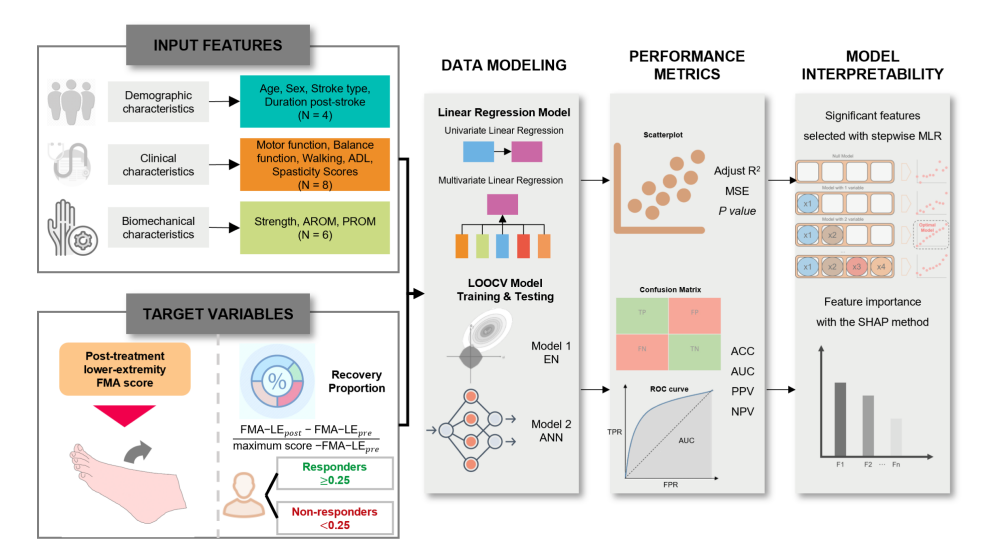
\includegraphics[
        width=\textwidth,
        height=0.75\textheight,
        keepaspectratio
    ]{Images/overall_framework.png}
    \caption{Overall Framework for Predicting Stroke Rehabilitation Outcomes Using Explainable AI}
    \label{fig:overall_framework}
\end{figure}


\section{{Step-by-Step Summary}}

\begin{enumerate}
    \item Collect baseline demographic, clinical, and biomechanical data from the patients.
    \item Conduct the two-week BCI-LE rehabilitation programme.
    \item Measure post-treatment lower-limb motor function using FMA-LE.
    \item Train regression models to estimate post-treatment FMA-LE scores.
    \item Calculate recovery proportions and classify patients as responders or non-responders.
    \item Train and evaluate Elastic Net and ANN classification models using LOOCV.
    \item Compare the models using ACC, AUC, PPV, and NPV.
    \item Apply stepwise regression and SHAP to identify important predictive features.
    \item Interpret the findings to understand factors associated with rehabilitation response.
\end{enumerate}

The above steps describe the methodology presented in the selected research paper. The study demonstrates how multimodal patient data, machine learning, and explainable AI can be combined to predict BCI rehabilitation outcomes and provide interpretable evidence that may support personalized treatment planning \cite{bib1}.
```